\documentclass[12pt]{article}

% AMS Packages
\usepackage{amsmath} 
\usepackage{amssymb} 
\usepackage{amsthm}

% Page dimensions
\usepackage[margin=0.9in]{geometry}

% Images
\usepackage[pdftex]{graphicx} 

% Enumerate package
\usepackage{enumitem} 
\usepackage{array} 

% Fancify pages
\usepackage{fancyhdr} 
%%% optional: add a header to the pages
\pagestyle{fancy}
\chead{}
\rhead{}
\lhead{}

% Convert captions on figures to bold font
\usepackage[labelfont=bf,textfont=md]{caption}

% Time New Roman font
\usepackage{times}

% change the line spacing
\usepackage{setspace} 

% SI Units in math type
\usepackage{siunitx}

% extra symbols
\usepackage{textcomp} 

\usepackage{wrapfig}

\usepackage{algorithm}
\usepackage[noend]{algpseudocode}
\makeatletter
\def\BState{\State\hskip-\ALG@thistlm}
\makeatother
% tikz 
\usepackage{tikz}
\usetikzlibrary{shapes.geometric, arrows}

% Change sizes of sections
\usepackage{titlesec}
\titleformat{\section}{\normalfont\large\bfseries}{\thesection}{1em}{}
\titleformat{\subsection}{\normalfont\bfseries}{\thesubsection}{1em}{}
\titleformat{\subsubsection}{\normalfont\small\bfseries}{\thesubsubsection}{1em}{}

% Declare useful math operators
\DeclareMathOperator*{\argmin}{arg\,min}
\DeclareMathOperator*{\plim}{plim}
\DeclareMathOperator{\Tr}{Tr}



\headsep 5pt


\begin{document}

\section{Introduction to Factor Analysis}
Factor analysis can be understood as a latent-linear generative model possessing the structure
\begin{align}
	\mathbf{X} &= \boldsymbol{\mu} + \mathbf{L} \mathbf{z} + \boldsymbol{\epsilon}
\end{align}
where 
\begin{itemize}
\item $\mathbf{X}$ constitutes the $N\times T$ observed data matrix;
\item $\boldsymbol{\mu}$ is the $N\times 1$ set of means for the $N$ unique features in the data matrix (the matrix is naturally broadcasted when we write the model formulation to encompass all $T$ data points).
\item  $\mathbf{L}$ is the $N\times K$ latent basis matrix (also called the loading matrix);
\item  $\mathbf{z}$ is the $K\times T$ matrix of latent factors (i.e. the coefficients of the latent representation); and
\item $\boldsymbol{\epsilon}$ is the $T\times N$ matrix of private noises.
\end{itemize}
Factor analysis, therefore, models the data as linearly arising from a $K$-dimensional, latent representation followed by a corruption of private noise.

Furthermore, factor analysis provides the data with an inherently Gaussian structure. The latent space, $\mathbf{z}$, takes on the simple form
\begin{align}
\mathbf{z} \sim \mathcal{N}(0, \mathbf{I})
\end{align}
and the private noise is similarly drawn from a Gaussian distribution with slightly different structure:
\begin{align}
\boldsymbol{\epsilon} \sim \mathcal{N}(0, \boldsymbol{\Psi}); \boldsymbol{\Psi} = \text{diag}\left(\Psi_1, \Psi_2, \ldots, \Psi_N\right).
\end{align}
Given this structure, a data point of $\mathbf{x}$ $(N\times 1)$ can be modeled in totality as a Gaussian distribution:
\begin{align}
	\mathbf{x} &\sim \mathcal{N}(\boldsymbol{\mu}, \boldsymbol{\Sigma}) \\
	\boldsymbol{\Sigma} &= \mathbf{LL}^T + \boldsymbol{\Psi}.
\end{align}
Thus, the factor analysis problem becomes: given a dataset $\mathbf{X} = \left\{\mathbf{x}^{(i)}\right\}_{i=1}^N$, what  $\mathbf{L}$ and $\boldsymbol{\Psi}$ sufficiently allow $\mathbf{X}$ to be described by the Gaussian model above?

\section{Maximum Likelihood}
Despite the fact that factor analysis is a latent model, we can still take a maximum likelihood approach to fit $\mathbf{L}$, $\boldsymbol{\Psi}$. To see this, note that the the log-likelihood can be written as 
\begin{align}
	\ell \left(\left\{\mathbf{x}^{(i)}\right\}_{i=1}^N|\mathbf{L}, \boldsymbol{\Psi}, \boldsymbol{\mu}\right) &= \sum_{i=1}^N \log p(\mathbf{x}^{(i)}) \\
	&= \sum_{i=1}^N \log \frac{1}{\sqrt{(2\pi)^N |\boldsymbol{\Sigma}|}} \exp\left[-\frac{1}{2} (\mathbf{x}^{(i)} - \boldsymbol{\mu})^T \boldsymbol{\Sigma}^{-1}\left(\mathbf{x}^{(i)} - \boldsymbol{\mu}\right)\right],
\end{align}
where, once again, $\boldsymbol{\Sigma}=\mathbf{LL}^T + \boldsymbol{\Psi}$. Simplifying the log-likelihood gives us
\begin{align}
\ell \left(\left\{\mathbf{x}^{(i)}\right\}_{i=1}^N|\mathbf{L}, \boldsymbol{\Psi}, \boldsymbol{\mu}\right) &= \sum_{i=1}^N -\frac{N}{2}\log(2\pi) -\frac{1}{2} \log\det \boldsymbol{\Sigma} - \frac{1}{2}(\mathbf{x}^{(i)} - \boldsymbol{\mu})^T \boldsymbol{\Sigma}^{-1}\left(\mathbf{x}^{(i)} - \boldsymbol{\mu}\right) \\
&= -\frac{N^2}{2} \log(2\pi) - \frac{N}{2} \log\det\boldsymbol{\Sigma} - \frac{1}{2}\sum_{i=1}^N(\mathbf{x}^{(i)} - \boldsymbol{\mu})^T \boldsymbol{\Sigma}^{-1}\left(\mathbf{x}^{(i)} - \boldsymbol{\mu}\right).
\end{align}
\subsection{Solving for $\boldsymbol{\mu}$}
First, note that maximizing the log-likelihood with respect to $\boldsymbol{\mu}$ is simple: taking the gradient gives us
\begin{align}
\partial_{\boldsymbol{\mu}} \ell \left(\left\{\mathbf{x}^{(i)}\right\}_{i=1}^N|\mathbf{L}, \boldsymbol{\Psi}, \boldsymbol{\mu}\right) &= -\frac{1}{2}\partial_{\boldsymbol{\mu}}  \sum_{i=1}^N(\mathbf{x}^{(i)} - \boldsymbol{\mu})^T \boldsymbol{\Sigma}^{-1}\left(\mathbf{x}^{(i)} - \boldsymbol{\mu}\right) \\
&= -\frac{1}{2} \cdot 2 \sum_{i=1}^N (\mathbf{x}^{(i)} - \boldsymbol{\mu})^T \boldsymbol{\Sigma}^{-1} \cdot \partial_{\boldsymbol{\mu}} (\mathbf{x}^{(i)} - \boldsymbol{\mu}) \\
&= \sum_{i=1}^N (\mathbf{x}^{(i)} - \boldsymbol{\mu})^T \boldsymbol{\Sigma}^{-1}.
\end{align}
Setting this equal to zero gives 
\begin{align}
\sum_{i=1}^N (\mathbf{x}^{(i)} - \boldsymbol{\mu})^T \boldsymbol{\Sigma}^{-1} &= \mathbf{0} \\
\Rightarrow \sum_{i=1}^N (\mathbf{x}^{(i)} - \boldsymbol{\mu}) &= \mathbf{0} \\
\Rightarrow \boldsymbol{\mu} = \frac{1}{N} \sum_{i=1}^N  \mathbf{x}^{(i)} &= \bar{\mathbf{x}},
\end{align}
as we might expect.
\subsection{Solving for $\mathbf{L}$}
With the solution for the mean, we can rewrite the log-likelihood as 
\begin{align}
	\ell \left(\left\{\mathbf{x}^{(i)}\right\}_{i=1}^N|\mathbf{L}, \boldsymbol{\Psi}\right) &= -\frac{N^2}{2} \log(2\pi) - \frac{N}{2} \log\det \boldsymbol{\Sigma} -\frac{1}{2} \sum_{i=1}^N(\mathbf{x}^{(i)} - \bar{\mathbf{x}})^T \boldsymbol{\Sigma}^{-1}\left(\mathbf{x}^{(i)} - \bar{\mathbf{x}}\right) \\
	&= -\frac{N^2}{2} \log(2\pi)- \frac{N}{2} \log\det \boldsymbol{\Sigma} -\frac{N}{2}\Tr\left[\mathbf{S} \boldsymbol{\Sigma}^{-1}\right] \\
	&= -\frac{N}{2} \left(N \log(2\pi) + \log\det \boldsymbol{\Sigma} + \Tr\left[\mathbf{S}\boldsymbol{\Sigma}^{-1}\right] \right).
\end{align}
Now, we assume that $\boldsymbol{\Psi}$ is already known (either we pick an initialization or we are improving on a current estimate); we will maximize the likelihood with respect to $\mathbf{L}$. Taking the gradient with respect to $\mathbf{L}$ gives us
\begin{align}
\partial_{\mathbf{L}} \ell \left(\left\{\mathbf{x}^{(i)}\right\}_{i=1}^N|\mathbf{L}, \boldsymbol{\Psi}, \boldsymbol{\mu}\right) &= -\Tr \left[\left(\partial_{\boldsymbol{\Sigma}} \log\det\boldsymbol{\Sigma}\right)^T \partial_{\mathbf{L}} \boldsymbol{\Sigma}\right] -\Tr \left[ \left(\partial_{\boldsymbol{\Sigma}} \Tr\left[\mathbf{S}\boldsymbol{\Sigma}^{-1}\right]\right)^T \partial_{\mathbf{L}} \boldsymbol{\Sigma}\right] \\
&= -\Tr\left[\boldsymbol{\Sigma}^{-1} \partial_{\mathbf{L}}\boldsymbol{\Sigma}\right] + \Tr \left[\boldsymbol{\Sigma}^{-1}\mathbf{S} \boldsymbol{\Sigma}^{-1} \partial_{\mathbf{L}} \boldsymbol{\Sigma}\right].
\end{align}
Setting this equal to 0 gives us 
\begin{align}
\Tr \left[\boldsymbol{\Sigma}^{-1}\mathbf{S} \boldsymbol{\Sigma}^{-1} \partial_{\mathbf{L}} \boldsymbol{\Sigma}\right] &= \Tr\left[\boldsymbol{\Sigma}^{-1} \partial_{\mathbf{L}}\boldsymbol{\Sigma}\right]
\end{align}
which can be achieved when 
\begin{align}
\boldsymbol{\Sigma}^{-1}\mathbf{S} \boldsymbol{\Sigma}^{-1} \partial_{\mathbf{L}}\boldsymbol{\Sigma} &= \boldsymbol{\Sigma}^{-1} \partial_{\mathbf{L}}\boldsymbol{\Sigma} \\
\Rightarrow \boldsymbol{\Sigma}^{-1} \mathbf{S} \boldsymbol{\Sigma}^{-1} \mathbf{L} &= \boldsymbol{\Sigma}^{-1} \mathbf{L}. 
\end{align}
We focus on the stationary point at 
\begin{align}
 \mathbf{L} &= \mathbf{S} \boldsymbol{\Sigma}^{-1} \mathbf{L}.
\end{align}
Now, according to the Woodbury matrix identity, we have
\begin{align}
	\boldsymbol{\Sigma}^{-1} &= (\boldsymbol{\Psi} + \mathbf{LL}^T)^{-1} \\
	&= \boldsymbol{\Psi}^{-1} - \boldsymbol{\Psi}^{-1} \mathbf{L} \left(\mathbf{I} + \mathbf{L}^T \boldsymbol{\Psi}^{-1} \mathbf{L} \right)^{-1} \mathbf{L}^T\boldsymbol{\Psi}^{-1}.
\end{align}
Thus,
\begin{align}
	\boldsymbol{\Sigma}^{-1} \mathbf{L} &= \boldsymbol{\Psi}^{-1}\mathbf{L} - \boldsymbol{\Psi}^{-1} \mathbf{L} \left(\mathbf{I} + \mathbf{L}^T \boldsymbol{\Psi}^{-1} \mathbf{L} \right)^{-1} \mathbf{L}^T\boldsymbol{\Psi}^{-1} \mathbf{L} \\
	&= \boldsymbol{\Psi}^{-1}\mathbf{L} \left[\mathbf{I} -  \left(\mathbf{I} + \mathbf{L}^T \boldsymbol{\Psi}^{-1} \mathbf{L} \right)^{-1} \mathbf{L}^T \boldsymbol{\Psi}^{-1}\mathbf{L}\right] \\
	&=  \boldsymbol{\Psi}^{-1}\mathbf{L} \left[\left(\mathbf{I} + \mathbf{L}^T \boldsymbol{\Psi}^{-1} \mathbf{L} \right)^{-1}\left(\mathbf{I} + \mathbf{L}^T \boldsymbol{\Psi}^{-1} \mathbf{L} \right) \right. \notag \\
	& \qquad \qquad -  \left.\left(\mathbf{I} + \mathbf{L}^T \boldsymbol{\Psi}^{-1} \mathbf{L} \right)^{-1} \mathbf{L}^T \boldsymbol{\Psi}^{-1}\mathbf{L}\right]\\
	&= \boldsymbol{\Psi}^{-1}\mathbf{L}\left(\mathbf{I} + \mathbf{L}^T \boldsymbol{\Psi}^{-1}\mathbf{L}\right)^{-1}.
\end{align}
Placing this expression in the condition for the stationary point gives us 
\begin{align}
	\mathbf{L} &= \mathbf{S} \boldsymbol{\Psi}^{-1}\mathbf{L}\left(\mathbf{I} + \mathbf{L}^T \boldsymbol{\Psi}^{-1}\mathbf{L}\right)^{-1} \\
	\Rightarrow \mathbf{L}\left(\mathbf{I} + \mathbf{L}^T \boldsymbol{\Psi}^{-1}\mathbf{L}\right) &= \mathbf{S}\boldsymbol{\Psi}^{-1} \mathbf{L}.
\end{align}

Now, we reparameterize the sample covariance matrix and the latent basis matrix according to
\begin{align}
	\tilde{\mathbf{L}} &\equiv \boldsymbol{\Psi}^{-1/2}\mathbf{L}\\
	\tilde{\mathbf{S}} &= \boldsymbol{\Psi}^{-1/2} \mathbf{S} \boldsymbol{\Psi}^{-1/2} 
\end{align}
so that the stationary point becomes
\begin{align}
	\tilde{\mathbf{L}}(\mathbf{I} + \tilde{\mathbf{L}}^T \tilde{\mathbf{L}}) &= \tilde{\mathbf{S}}\tilde{\mathbf{L}}.
\end{align}
Consider the thin SVD decomposition of $\tilde{\mathbf{L}}$, in which we only consider the first $K$ singular values:
\begin{align}
	\tilde{\mathbf{L}} &= \mathbf{U}_K \mathbf{D}_K \mathbf{V}^T.
\end{align}
To be clear, the dimensionalities in the thin SVD are $\dim(\mathbf{U}_K) = N\times K$, $\dim(\mathbf{D}_K) = K\times K$, and $\dim(V) = K\times K$. In addition, with have the usual orthonormality properties of SVD. Placing the SVD into the stationary point condition gives us
\begin{align}
	\mathbf{U}_K \mathbf{D}_K \mathbf{V}^T \left(\mathbf{I} + \mathbf{V} \mathbf{D}_K^2 \mathbf{V}^T\right) &= \tilde{\mathbf{S}} \mathbf{U}_K \mathbf{D}_K \mathbf{V}^T \\
	\Rightarrow \mathbf{U}_K \mathbf{D}_K \mathbf{V}^T + \mathbf{U}_K \mathbf{D}_K^3 \mathbf{V}^T &=  \tilde{\mathbf{S}} \mathbf{U}_K \mathbf{D}_K \mathbf{V}^T \\
	 \Rightarrow \mathbf{U}_K + \mathbf{U}_K \mathbf{D}_K^2 &= \tilde{\mathbf{S}} \mathbf{U}_K \\
	 \Rightarrow \mathbf{U}_K \left(\mathbf{I} + \mathbf{D}_K^2\right) &= \tilde{\mathbf{S}} \mathbf{U}_K.
\end{align}
This equation is a natural eigenvalue equation for the matrix $\tilde{\mathbf{S}}$; to make this clear, we can rewrite it in terms of the $j$th left singular vector $\mathbf{u}_K^{(j)}$:
\begin{align}
\tilde{\mathbf{S}} \mathbf{u}_K^{(j)} &= \left[1 + \left(d_K^{(j)}\right)^2\right] \mathbf{u}_K^{(j)}.
\end{align}
Thus, the left singular vectors are just  eigenvectors of the reparameterized covariance matrix. We see, then, how this approach for Factor Analysis invokes Principal Components Analysis. 

Let us remind ourselves where we came from: we defined a reparameterization of the desired quantity, $\mathbf{L}$, as 
\begin{align}
	\tilde{\mathbf{L}} &= \boldsymbol{\Psi}^{-1/2} \mathbf{L}  \\
	\Rightarrow \mathbf{L} &= \boldsymbol{\Psi}^{1/2} \tilde{\mathbf{L}}.
\end{align}
Furthermore, we now know the SVD of the reparameterization. So, 
\begin{align}
	\mathbf{L} &= \boldsymbol{\Psi}^{1/2} \mathbf{U}_K \left(\boldsymbol{\Lambda}_K - \mathbf{I}\right)^{1/2} \mathbf{V}^T
\end{align}
where $\boldsymbol{\Lambda}_K$ is the diagonal matrix of the largest $K$ eigenvalues corresponding to the eigendecomposition of $\tilde{\boldsymbol{S}}$. Similarly, $\mathbf{U}_K$ are the corresponding $K$ eigenvectors. Interestingly, note that by the unitarity of $\mathbf{V}$, we can simply write
\begin{align}
	\mathbf{L} \leftarrow \mathbf{L}\mathbf{V} &= \boldsymbol{\Psi}^{1/2} \mathbf{U}_K \left(\boldsymbol{\Lambda}_K - \mathbf{I}\right)^{1/2} \mathbf{V}^T \mathbf{V} \\
	&= \boldsymbol{\Psi}^{1/2} \mathbf{U}_K \left(\boldsymbol{\Lambda}_K - \mathbf{I}\right)^{1/2}
\end{align}
since the likelihood is invariant under rotations of $\mathbf{L}$. 

This process involves computing the eigendecomposition of a transformed sample covariance matrix. Rather than having to take the intermediate step of calculating $\hat{\mathbf{S}}$, we simply note that the thin SVD of 
\begin{align}
	\tilde{\mathbf{X}} &= \frac{1}{\sqrt{N}} \boldsymbol{\Psi}^{-1/2} \mathbf{X} \\
	&= \mathbf{U}_H \sqrt{\boldsymbol{\Lambda}_K} \tilde{\mathbf{W}}^T
\end{align}
where $\mathbf{X}$ has already been centered.
\section{Proposed ``Iterated'' Factor Analysis Method}

For a data matrix $\mathbf{X}^{(0)}$ ($\dim(X) = N\times T$) our proposed Factor Analysis procedure is as follows:
\begin{itemize}
	\item For $k$ from $1$ to $\hat{K}$ (potentially identified by some stopping criteria):
	\begin{enumerate}[label=\textbf{(\arabic*)}]
		\item Perform Factor Analysis (e.g. using the SVD based approach above) assuming $K=1$. Call the fitted latent factor $\mathbf{L}^{(k)}$ and private variability $\boldsymbol{\Psi}^{(k)}$.
		\item Project the data matrix down to the latent space according to the expectation update (from the EM-algorithm):
		\begin{align}
			\langle \mathbf{z} \rangle_{p(\mathbf{z}|\mathbf{X})}^{(k)} &= \left(\mathbf{I} +{\mathbf{L}^{(k)}}^T {\boldsymbol{\Psi}^{(k)}}^{-1}\mathbf{L}^{(k)}\right)^{-1} {\mathbf{L}^{(k)}}^T {\boldsymbol{\Psi}^{(k)}}^{-1} \mathbf{X}^{(k-1)}.
		\end{align}
		\item Produce a modified dataset, $\mathbf{X}^{(k)}$, obtained by subtracting out the shared variability:
		\begin{align}
			\mathbf{X}^{(k)} &= \mathbf{X}^{(k-1)} - \mathbf{L}^{(k)} \langle \mathbf{z} \rangle^{(k)} \\
			&= \left[\mathbf{I} - \mathbf{L}^{(k)} \left(\mathbf{I} +{\mathbf{L}^{(k)}}^T {\boldsymbol{\Psi}^{(k)}}^{-1}\mathbf{L}^{(k)} \right)^{-1} {\mathbf{L}^{(k)}}^T {\boldsymbol{\Psi}^{(k)}}^{-1}\right] \mathbf{X}^{(k-1)}  \\
			&= \boldsymbol{\Psi}^{(k)}\left[\boldsymbol{\Psi}^{(k)} + \mathbf{L}^{(k)}{\mathbf{L}^{(k)}}^T\right]^{-1} \mathbf{X}^{(k-1)}.
		\end{align}
	\end{enumerate}
	\item Create the full latent basis matrix $\mathbf{L}$ according to
	\begin{align}
		\mathbf{L} &= \left(\begin{array}{cccc}
			\vline & \vline & \cdots & \vline \\
			\mathbf{L}^{(1)} & 	\mathbf{L}^{(2)} & \cdots & 	\mathbf{L}^{(\hat{K})}\\
			\vline & \vline & \cdots & \vline 
		\end{array}\right)
	\end{align}
	and the private variability according to the maximum likelihood result
	\begin{align}
		\boldsymbol{\Psi} &= \text{diag}\left(\mathbf{S} - \mathbf{LL}^T\right)
	\end{align}
	where $\mathbf{S}$ is the sample covariance matrix. Importantly, we only need the diagonal of the covariance matrix which amounts to calculating the variance of each feature in $\mathbf{X}$.
\end{itemize}
Because our method only performs Factor Analysis with one latent component, each step is akin to finding the principal value and its corresponding principal component of the scaled data matrix. 

\section{Experiments}
Below, we compare the performance of normal factor analysis (gray) to iterated factor analysis (red) on both training and test sets. Normal factor analysis is plotted against number of components, while iterated factor analysis is plotted against number of iterations. Iterated factor analysis achieves equal or better performance on the log-likelihood. 
\begin{figure}[H]
	\centering
	\scalebox{0.17}{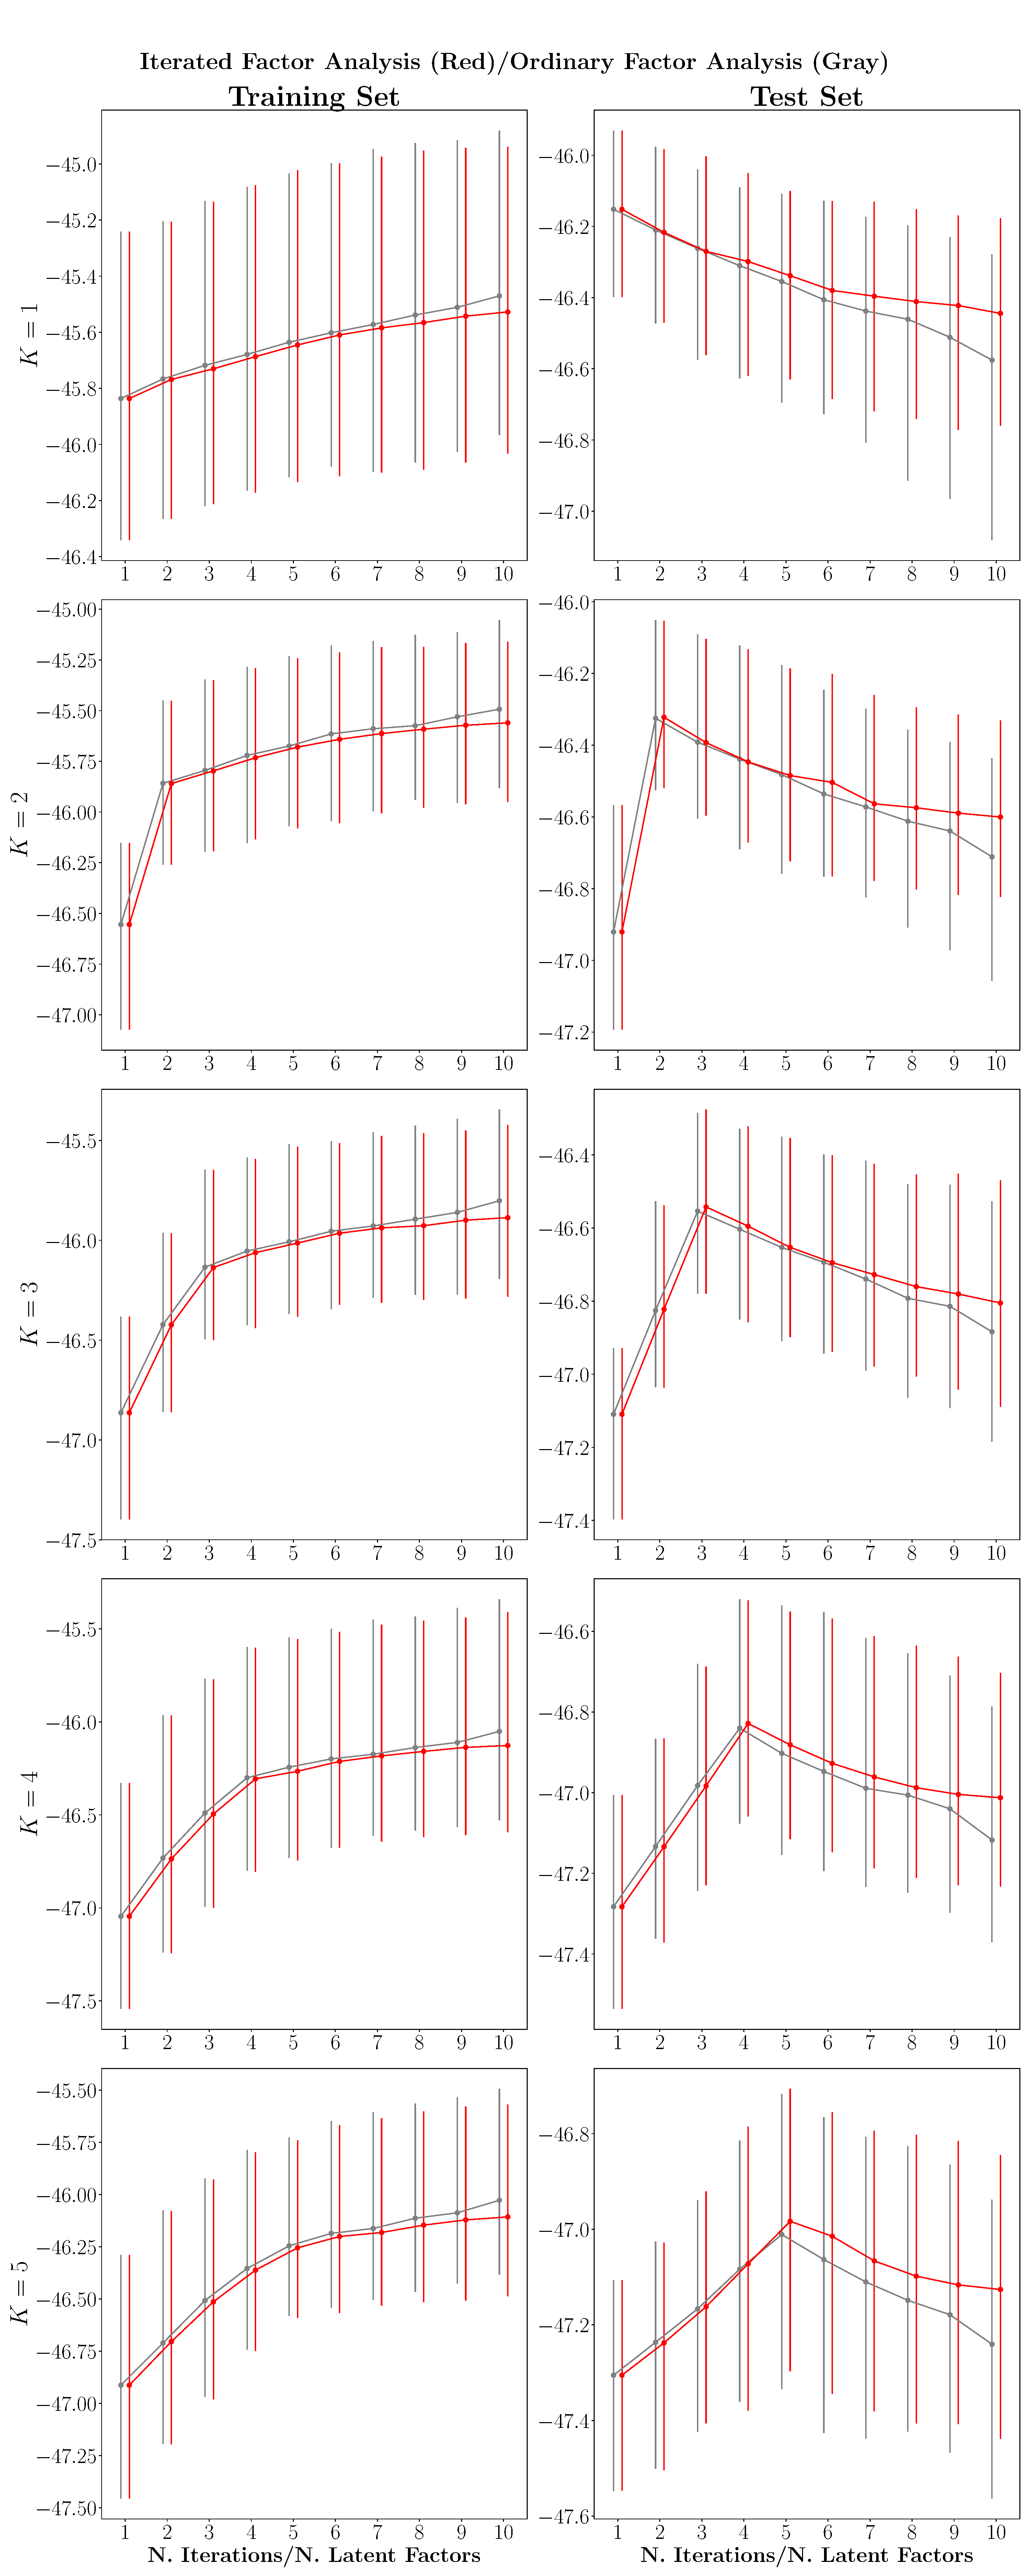
\includegraphics{img/iter_vs_vanilla_fa.pdf}}
\end{figure}
\newpage
\section{Algorithms}
\begin{algorithm}
	\caption{\textsc{FactorAnalysisSVD}$(\mathbf{X}, K)$}\label{euclid}
	\begin{algorithmic}[1]
		\State Initialise diagonal noise $\boldsymbol{\Psi}$
		\State Center the data matrix $\mathbf{X}$.
		\State Compute the variance $\mathbf{v} = \left\{v_i\right\}_{i=1}^N$ across each feature $\mathbf{x}_i$.
		\While{Likelihood not converged according to stopping criterion}
		\State Scale the data matrix $\tilde{\mathbf{X}} = \boldsymbol{\Psi}^{-1/2} \mathbf{X}/\sqrt{N}$.
		\State Perform SVD on $\tilde{\mathbf{X}} = \tilde{\mathbf{U}}\tilde{\boldsymbol{\Lambda}}\tilde{\mathbf{W}}^T$.
		\State $\mathbf{U}_K \leftarrow$ first $K$ columns of $\mathbf{U}$
		\State $\mathbf{\Lambda}_K \leftarrow$ first $K$ diagonal entries of $\tilde{\boldsymbol{\Lambda}}$.
		\State $\mathbf{L} = \boldsymbol{\Psi}^{1/2} \mathbf{U}_K(\boldsymbol{\Lambda}_K - \mathbf{I}_K)^{1/2}.$
		\State Update the log-likelihood.
		\State $\boldsymbol{\Psi} = \text{diag}(\mathbf{v}) - \text{diag}(\mathbf{LL}^T)$.
		\EndWhile
		\State
		\Return $\mathbf{L}$, $\boldsymbol{\Psi}$
	\end{algorithmic}
\end{algorithm}
\begin{algorithm}
	\caption{\textsc{IteratedFA}$(\mathbf{X}, K)$}\label{euclid}
	\begin{algorithmic}[1]
		\State Center the data matrix $\mathbf{X}^{(0)}$.
		\State Compute the variance $\mathbf{v} = \left\{v_i\right\}_{i=1}^N$ across each feature $\mathbf{x}_i$.
		\For{Iteration $k$ until stopping criterion}
		\State $\mathbf{L}^{(k)}, \boldsymbol{\Psi}^{(k)}=$ \textsc{FactorAnalysisSVD}($\mathbf{X}^{(k)}, 1)$
		\State Subtract out shared variability: $\mathbf{X}^{(k+1)} = \boldsymbol{\Psi}^{(k)}\left[\boldsymbol{\Psi}^{(k)} + \mathbf{L}^{(k)}{\mathbf{L}^{(k)}}^T\right]^{-1} \mathbf{X}^{(k-1)}$
		\State Store $\mathbf{L}^{(k)}$.
		\EndFor
		\State $\mathbf{L}=\left(\mathbf{L}^{(1)} \ \mathbf{L}^{(2)} \ \cdots \mathbf{L}^{(K)}\right)$.
		\State $\boldsymbol{\Psi} = \text{diag}(\mathbf{v}) - \text{diag}(\mathbf{LL}^T)$.
		\State
		\Return $\mathbf{L}$, $\boldsymbol{\Psi}$
	\end{algorithmic}
\end{algorithm}
\end{document}